
\begin{figure}[htbp]
  \centering
  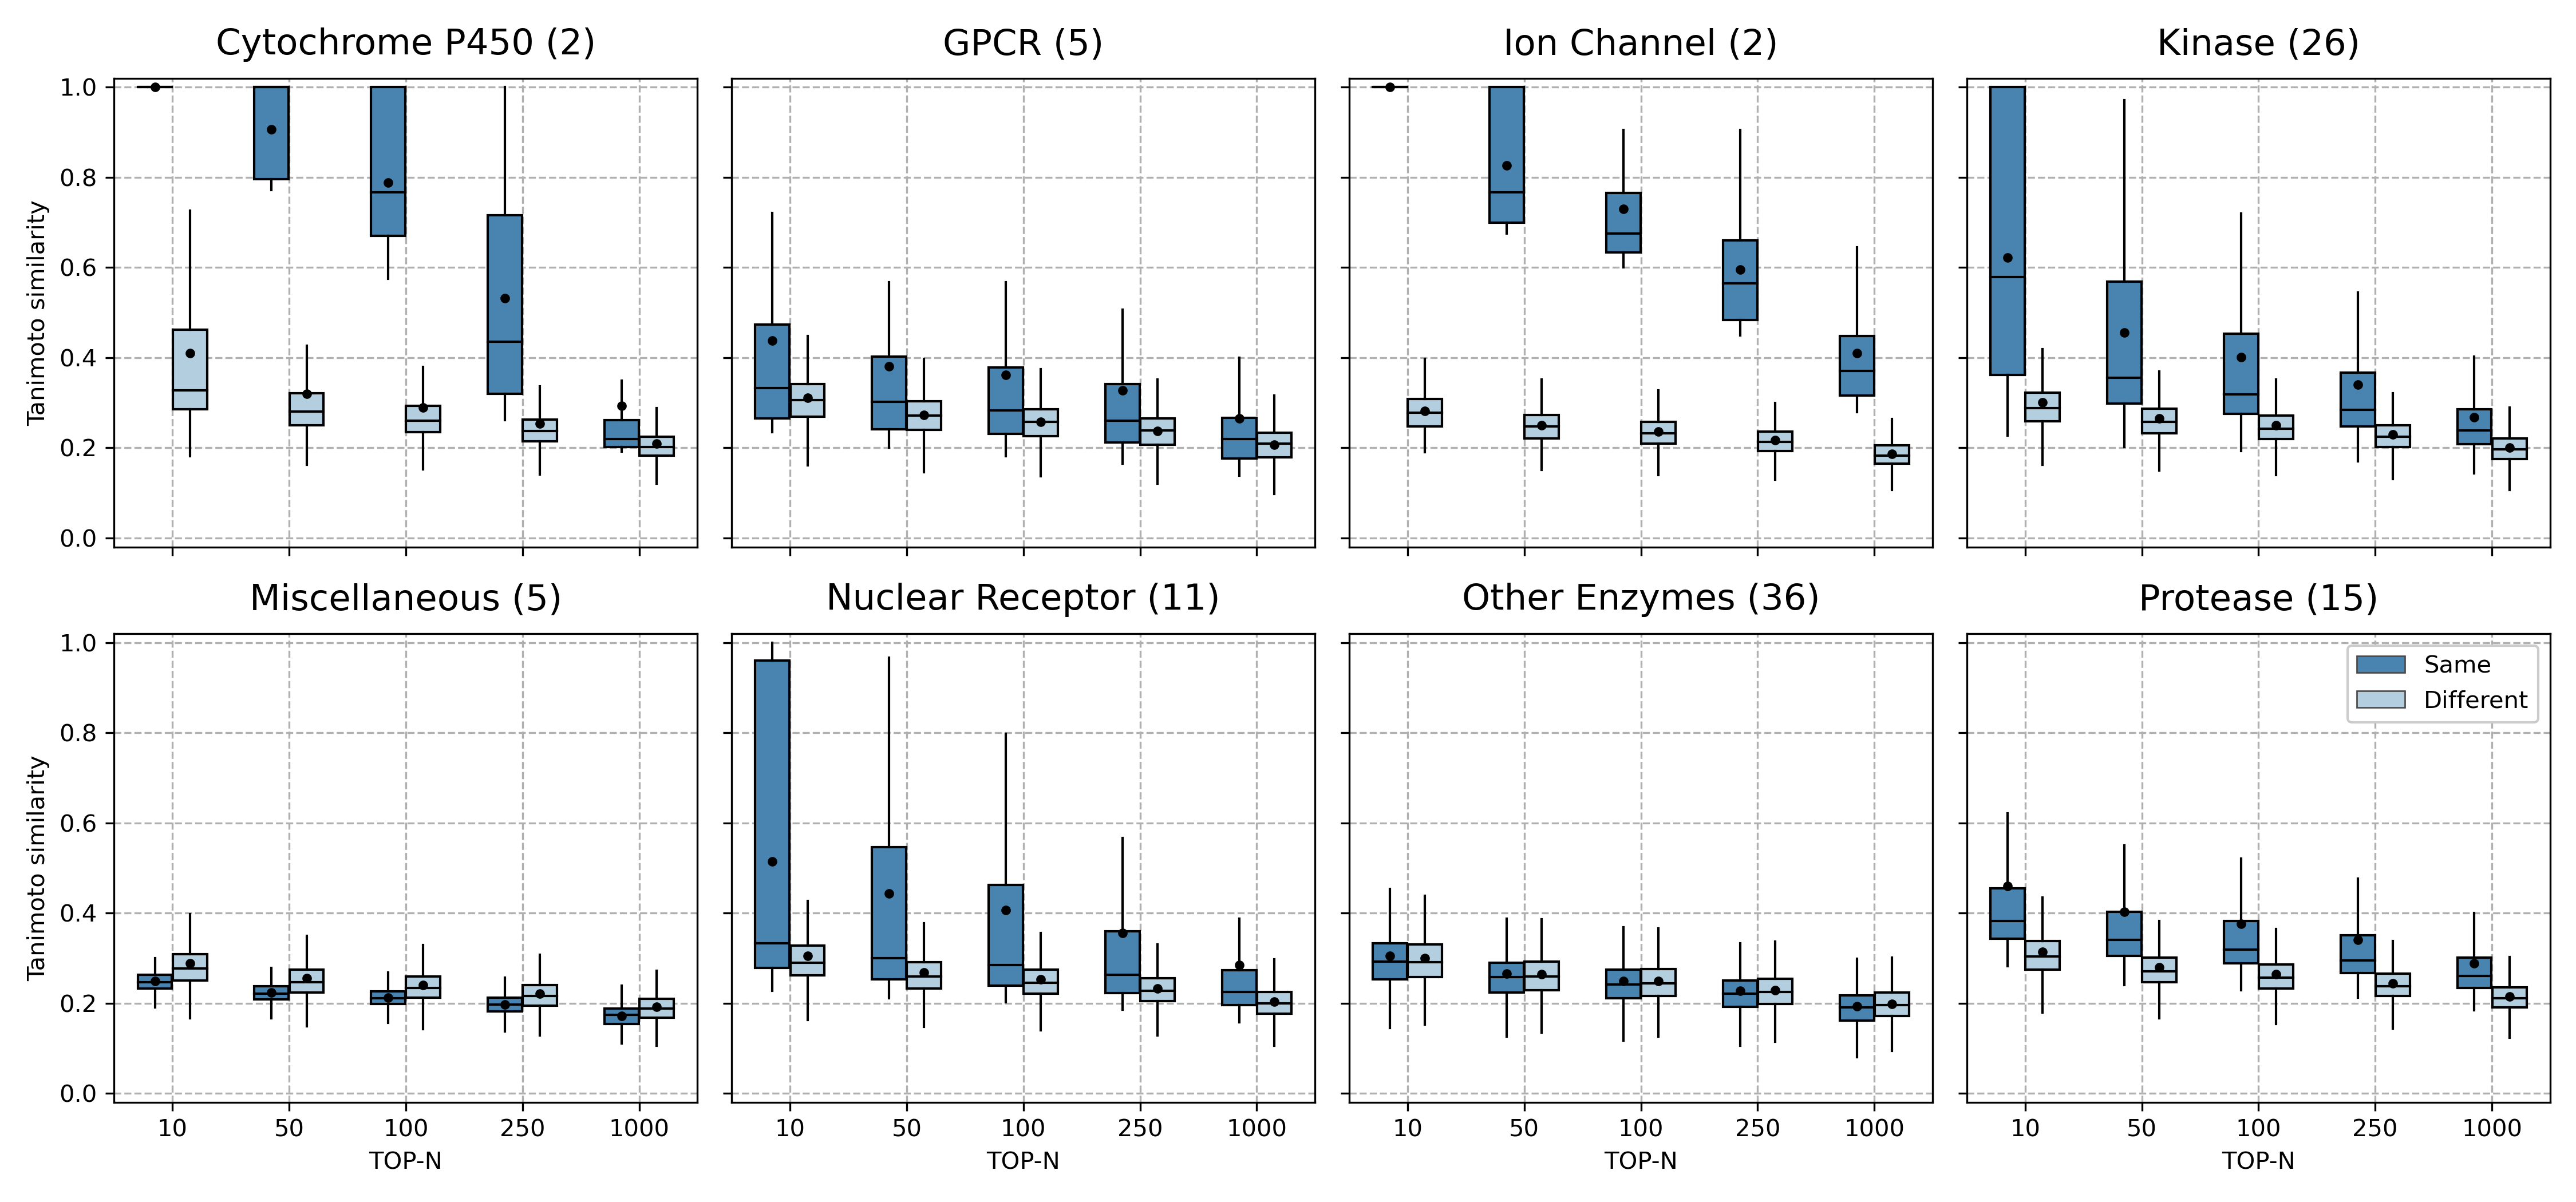
\includegraphics[width=\linewidth]{figures/PocketVec/Supplementary/FigS1.png}
  \caption{Similar proteins bind similar active compounds. For each protein family (e.g. Cytochrome P450, GPCR, etc.) we compared all active compounds between protein pairs from the same family (Same) and from different families (Different). Compounds were compared on the basis of their Tanimoto Similarities (y-axis, ECFP4 with 2048 bits using RDKit – https://rdkit.org) and only the TOP-N (x-axis: 10, 50, 100, 250, 1000) highest similarities were considered per each family. All distributions of Same and Different categories are significantly different (Mann-Whitney U test, pvalue <0.05, alternative greater using SciPy\cite{virtanen_scipy_2020}) except Miscellaneous (10, 50, 100, 250, 1000) and Other Enzymes (10, 50, 100, 250, 1000). Box plots indicate median (middle line), 25th, 75th percentile (box), and max and min value within the 1.5*25th and 1.5*75th percentile range (whiskers). Black dots represent mean values. The number of proteins within each family is specified in the title in parenthesis. Data was downloaded from http://dude.docking.org in January 2023.}
  \label{fig:example-figure}
\end{figure}